\documentclass[crop,tikz]{standalone}                 
\usepackage{physics}

\makeatletter                                                                                        

\newcommand{\sq}[1]{\frac{1}{\sqrt{#1}}}

\begin{document}

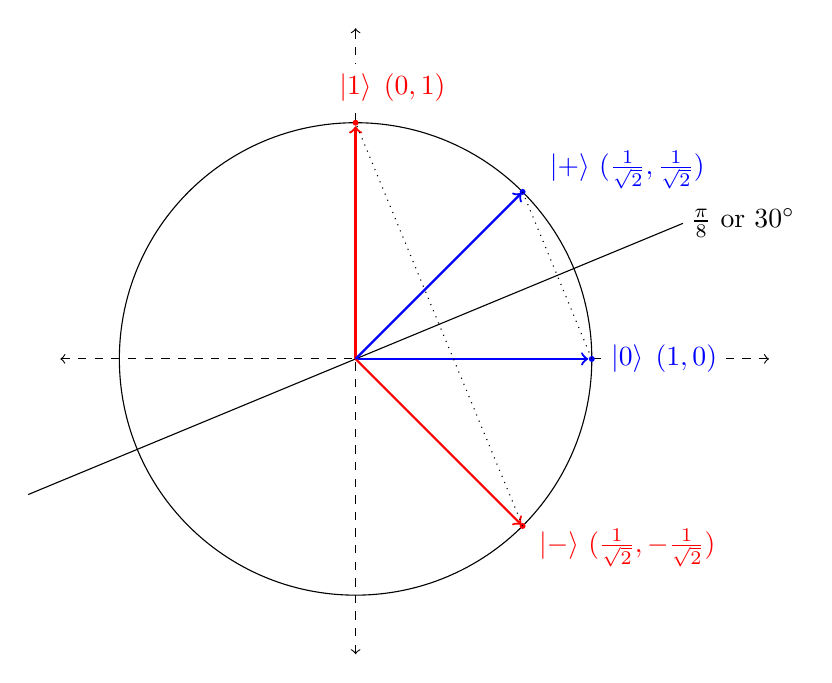
\begin{tikzpicture}[scale=1.5]                                                                          
\usetikzlibrary{positioning}
%\draw [dashed,gray, step=2cm] (-2.30,-2.30) grid ( 2.30, 2.30);

% Axes
\draw [-] (-2.77164,-1.14805) -- (2.77164,1.14805);
\draw [<->, dashed] (0,-2.5) -- (0,2.8);
\draw [<->, dashed] (-2.5, 0) -- (3.5,0);

% Circle
\draw[] (0cm,0cm) circle(2.00cm);                                                                 

% Point ket-1
\filldraw[red] (0.00,2.00) circle (0.02cm);
\draw [->,thick,red] (0,0) -- (0.00, 1.97);
\node [fill=white,text=red] (ket1) at ( 0.00, 2.30) {$\ket{1}$};
\node [red]             (al) at ( 0.50, 2.30) {$(0,1)$};

% Point ket-0
\filldraw[blue] ( 2.00, 0.00) circle (0.02cm);
\draw [->,thick,blue] (0,0) -- (1.97, 0.00);
\node [fill=white,text=blue] (ket2) at ( 2.30, 0.00) {$\ket{0}$};
\node [fill=white, text=blue]             (al) at ( 2.80, 0.00) {$(1,0)$};

% Point ket-minus
\filldraw[red] (1.41421,-1.41421) circle (0.02cm);
\draw [->,thick,red] (0,0) -- (1.40421, -1.40421);
\node [text=red] (ket3) at ( 2.3, -1.60) {$\ket{-}$  $(\frac{1}{\sqrt{2}},-\frac{1}{\sqrt{2}})$};

% Point ket-minus
\filldraw[blue] (1.41421, 1.41421) circle (0.02cm);
\draw [->,thick,blue] (0,0) -- (1.40421, 1.40421);
\node [text=blue] (ket4) at ( 2.3, 1.60) {$\ket{+}$  $(\frac{1}{\sqrt{2}}, \frac{1}{\sqrt{2}})$};

% Reflection Lines
\draw [-,dotted] (1.41421,-1.41421) -- (0.00,2.00);
\draw [-,dotted] (1.41421, 1.41421) -- (2.00,0.00);

% Angle
\node [] (angle) at ( 3.28, 1.15) {$\frac{\pi}{8}$ or $30^{\circ}$};


\end{tikzpicture}                                                                                    

\end{document}
